\RussianSourceFrame{GELFAND-P001485}{87}

\begin{equation*}
\int \mathcal{D}x\,e^{mL}
\longrightarrow
\int \mathcal{D}x\,\mathcal{D}\lambda\,
e^{\int \lambda^{-1}\dot{x}^{2}\,dt+\int m\lambda\,dt}
\tag{10}
\end{equation*}
[Перед $m\lambda\,dt$ зачёркнуто:
\RussianUnclear{GELFAND-P001485}{eq10-cancellation}{неразборчивый знак, возможно $m$}.]

$L$ как в (5)

Интегрир. методом перевала справа (по $\lambda$), получаем
$\lambda^{2}=\dfrac{\dot{x}^{2}}{m^{2}}$.

\begin{equation*}
\int \mathcal{D}x\,e^{m\int\sqrt{\dot{x}^{2}}\,dx}
\tag{11}
\end{equation*}
\RussianUnclear{GELFAND-P001485}{eq11-differential}{В конце показателя: $dx$; возможно $dt$.}

((11) $\Rightarrow$ (10) избавляет от корня). Оказ., что равенство точное!!

Число $\lambda$ имеет смысл 1-мерн. метрики
(всё остальное \RussianUnclear{GELFAND-P001485}{metric-abbreviation}{свод. / своб.}
из репараметризации)

\begin{equation*}
\int\frac{d\lambda}{\lambda}\,e^{a\lambda}e^{b/\lambda}
=e^{\sqrt{ab}}
\tag{12}
\end{equation*}
\RussianUnclear{GELFAND-P001485}{eq12-identity}{Равенство с $e^{\sqrt{ab}}$ без дополнительных множителей.}

Грин и др. сделали аналог. вещь в теор. струн: переход к

\begin{equation*}
\sum_{\text{топол.}}\int\mathcal{D}x\,\mathcal{D}g\,
e^{\int\sqrt{g}\,g^{ab}\partial_a x^{\mu}\partial_b x^{\mu}\,d\sigma\,dt}
\underbrace{e^{\int\sqrt{g}\,d\sigma\,dt}}_{\text{это можно убрать}}
\tag{13}
\end{equation*}

\underline{Обобщение:}

кривое 26-мерн. пр-во

\begin{equation*}
\begin{aligned}
\sum_{\text{топол.}}\int\mathcal{D}x\,\mathcal{D}g\,
e^{\int G_{\mu\nu}(x)\sqrt{g}\,g^{ab}\partial_a x^{\mu}\partial_b x^{\nu}}
&{}\\
&d\sigma\,dt
\end{aligned}
\tag{14}
\end{equation*}
\RussianUnclear{GELFAND-P001485}{eq14-differentials}{Множитель $d\sigma\,dt$ написан ниже показателя экспоненты; принадлежность показателю неясна.}

Хотим, чтобы вып. ур-я Эйнштейна

\begin{equation*}
R_{\mu\nu}(x)=0
\tag{15}
\end{equation*}

\begin{equation*}
\begin{gathered}
(15)\ \Leftrightarrow\ \text{дилатационная инвариантность!}\\
\Downarrow\\
\text{ур-я Янга Миллса}
\end{gathered}
\end{equation*}

Все инвар. ур-я для высших полей — следствие дилат.
инвар. (в однопетлевом приближении)


\RussianSourceFrame{GELFAND-P001486}{unlabelled}

\underline{$26/\overline{\underline{\mathrm{IX}}}$-88 г.}
\qquad \underline{\underline{Сем. Гельфанда.}}

\underline{И.М.Г.} Читать кн. Фейнмана о КЭД и
\RussianUnclear{GELFAND-P001486}{feynman-verb}{учить / учите / учиться}
\RussianUnclear{GELFAND-P001486}{feynman-noun}{эстетике / эстетику}
у него.

Там КЭД изложена без ф-л — на одних картинках.

\underline{\underline{Казаков.}}
\quad \underline{Комбинаторика и новые раб. по струнам}

Произошли события (в комбинаторике)

\underline{Поляков} и
[зачёркнуто: \RussianUnclear{GELFAND-P001486}{names-cancellation}{по?}]
\underline{Замолодчиков — Книжник — Поляков}
показали, что действит. модели, прив. выше, опис. 2-мерную
квант. гравитацию.

(Книжник — Поляков — Замолодчиков)

[Под именами:] по англ. алфавиту.

З.-К.-П. рассмотрели модель бозонной струны.

\begin{equation*}
S=\int d^{2}\xi\,\sqrt{g}\,\partial_a x^{\mu}\partial_b x^{\mu}\,g^{ab}
+\beta\int d^{2}\xi\,\sqrt{g}
\tag{1}
\end{equation*}

\begin{equation*}
Z(\beta)=\int\mathcal{D}g_{ab}\int\mathcal{D}x^{\mu}\,e^{-S}
\tag{2}
\end{equation*}

$\mu=1,\ldots,D$.

\RussianSourceFigure{GELFAND-P001486}{metric-diagram}{Внизу справа две пересекающиеся примерно перпендикулярные оси: горизонтальная с подписью $\xi_1$ справа и вертикальная с подписью $\xi_2$ слева вверху. Справа от вертикальной оси, над горизонтальной, расположен замкнутый неровный контур, внутри которого написано $g_{ab}(\xi)$. Направления наконечников осей неуверенно различимы.}

\par\medskip\noindent
\begin{minipage}[c]{0.48\linewidth}\centering
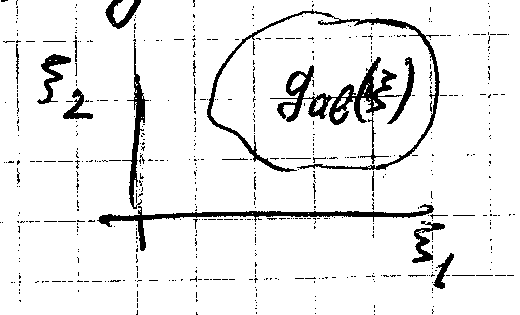
\includegraphics[width=\linewidth]{figures/gelfand-p001486-metric-diagram-original.png}
\par\smallskip{\footnotesize Оригинал рукописного рисунка: GELFAND-P001486\par}
\end{minipage}\hfill
\begin{minipage}[c]{0.48\linewidth}\centering
\resizebox{\linewidth}{!}{% Partial visible-stroke recreation. Endpoint hooks do not assert arrows; gaps remain open.
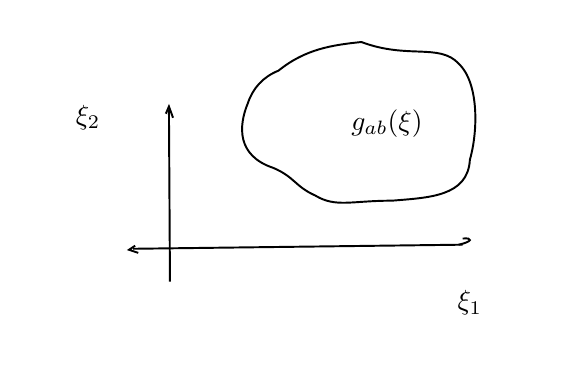
\begin{tikzpicture}[x=0.013cm,y=-0.013cm,line width=0.7pt]
\path[use as bounding box] (0,0) rectangle (520,315);
\draw (139,248)--(138,80);\draw (135,84)--(138,77)--(142,88);
\draw (103,216)--(425,212);\draw (105,213)--(99,217)--(108,220);
\draw (421,212)..controls(435,209)and(435,205)..(425,206);
\draw (245,42)..controls(271,21)and(297,17)..(326,14)
 ..controls(371,31)and(402,15)..(421,35)
 ..controls(441,54)and(440,101)..(432,129)
 ..controls(430,165)and(392,166)..(356,169)
 ..controls(316,169)and(301,176)..(281,164)
 ..controls(261,155)and(261,146)..(240,137)
 ..controls(204,125)and(206,96)..(215,74)
 ..controls(220,59)and(230,48)..(245,42);
\node at (59,88) {$\xi_2$};\node at (432,269) {$\xi_1$};
\node at (351,94) {$g_{ab}(\xi)$};
\end{tikzpicture}
}
\par\smallskip{\footnotesize Частичное воссоздание; неясные направления и соединения остаются неустановленными.\par}
\end{minipage}\par\medskip



\RussianSourceFrame{GELFAND-P001487}{unlabelled}

Интеграл (2) опр. при
\RussianUnclear{GELFAND-P001487}{top-beta-inequality}{$\beta>\beta_c$ / $\beta\ge\beta_c$; знак переправлен}
и там ведёт себя как
\begin{equation*}
(\beta-\beta_c)^{2-\gamma_{\mathrm{str}}(D)}
\tag{3}
\end{equation*}

(в $\beta_c$ объём пов. стан. беск.)

[Над строкой: $\mathrm{str}=\mathrm{string}$.]

К.-П.-З. доказали, что
\begin{equation*}
\gamma_{\mathrm{str}}=\frac{1}{12}
\left(D-1-\sqrt{(D-1)(D-25)}\right).
\tag{4}
\end{equation*}

Это имеет смысл при
\RussianUnclear{GELFAND-P001487}{upper-dimension-range}{$D\le1$ и $D\ge26$ [так в источнике]}.
Это получено с пом. алгебр Каца-Муди, возникших у исслед.
Лагранжиана.

\underline{Казаков и др.} предсказали неск. значений $\gamma_{\mathrm{str}}$:
при $D=-2,0,\frac12,1$

[На левом поле:
\RussianUnclear{GELFAND-P001487}{left-margin-monogram}{ИГ / ИМ?}.]
Всё совпало!!

Определим:
\begin{equation*}
Z(\beta)=\sum_{n=0}^{\infty}e^{-2n\beta}Z_{2n},
\tag{5}
\end{equation*}
где $Z_n$ — число планарных графов
[вставлено над строкой: с $n$ вершинами]
с топологией сферы
(в вершине должны сход. 3 ребра)

Тогда
\begin{equation*}
Z(\beta)\sim(\beta-\beta_c)^{2-\gamma_{\mathrm{str}}(D)}
\tag{6}
\end{equation*}
[Над $\gamma_{\mathrm{str}}(D)$ проведена скобка; справа от неё: $=-\frac12$.]
Это соответствует $D=0$

\RussianSourceFigure{GELFAND-P001487}{right-margin-triangle-graphs}{На правом поле два рисунка один под другим. В верхнем рисунке большой треугольник с верхней вершиной и горизонтальным основанием; внутри меньший треугольник той же ориентации. Каждая вершина внутреннего треугольника соединена с соответствующей внешней вершиной. На нижней стороне внутреннего треугольника около левой вершины есть утолщение, похожее на наконечник влево; у правой нижней внешней вершины есть штрихи, похожие на наконечник вправо. В нижнем рисунке внешний треугольник и три отрезка от его вершин к внутренней точке; отрезок от левой нижней вершины не вполне доходит до точки соединения двух других отрезков. Буквенных или числовых подписей у этих двух рисунков нет. Требуют проверки наконечники и смысл разрыва в нижнем рисунке.}

\par\medskip\noindent
\begin{minipage}[c]{0.48\linewidth}\centering
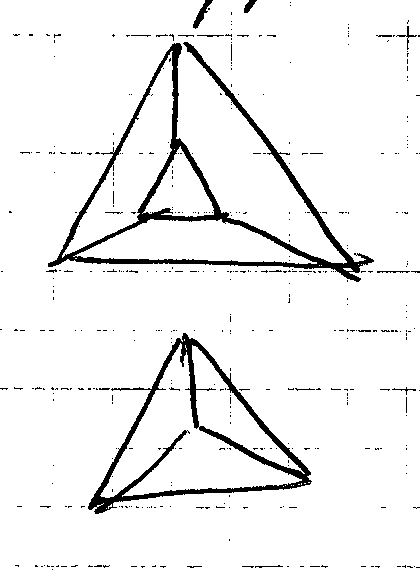
\includegraphics[width=\linewidth]{figures/gelfand-p001487-right-margin-triangle-graphs-original.png}
\par\smallskip{\footnotesize Оригинал рукописного рисунка: GELFAND-P001487\par}
\end{minipage}\hfill
\begin{minipage}[c]{0.48\linewidth}\centering
\resizebox{\linewidth}{!}{% Partial visible-stroke recreation. Endpoint hooks do not assert arrows; gaps remain open.
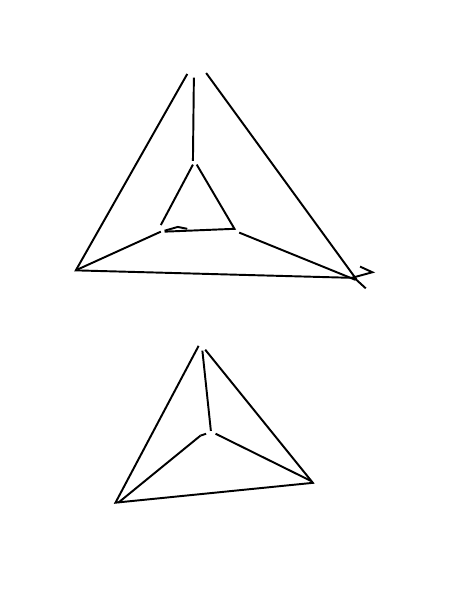
\begin{tikzpicture}[x=0.012cm,y=-0.012cm,line width=0.7pt]
\path[use as bounding box] (0,0) rectangle (420,570);
\draw (169,49)--(51,257)--(347,265)--(189,48);
\draw (176,53)--(175,141);\draw (175,145)--(141,209);
\draw (179,145)--(219,213)--(145,216);\draw (141,216)--(53,256);
\draw (224,217)--(347,267);\draw (145,215)--(159,211)--(169,213);
\draw (343,265)--(365,259)--(352,253);\draw (347,266)--(358,276);
\draw (181,337)--(93,503)--(302,482)--(188,341);
\draw (185,342)--(194,427);\draw (199,430)--(300,480);
\draw (96,503)--(183,432);\draw (183,432)--(189,430);
\end{tikzpicture}
}
\par\smallskip{\footnotesize Частичное воссоздание; неясные направления и соединения остаются неустановленными.\par}
\end{minipage}\par\medskip


[Зачёркнуто:
\RussianUnclear{GELFAND-P001487}{middle-cancelled-word}{число?}.]
Асимптотика
\begin{equation*}
Z_{2n}\sim\left(\frac{256}{27}\right)^n n^{-3+\gamma_{\mathrm{str}}}
\tag{7}
\end{equation*}

$\gamma_{\mathrm{str}}$ — универс. число, не зав. от способа опр. план. графов
(можно 4 ребра в 1 вершине и т. п.)

\underline{Формула для $Z_n$.}

[Перед оставленной правой частью (8) зачёркнута дробь:
\RussianUnclear{GELFAND-P001487}{bottom-cancelled-fraction}{$2\frac{(4n+7)!}{(n-4)}$ / $2\frac{(4n+1)!}{(n-4)}$ / $2\frac{(4n-7)!}{(n-4)}$; $n$ либо $k$, факториал в знаменателе неясен}.]
\begin{equation*}
Z_{2k}=2\frac{(4k-3)!}{(3k-1)!\,k!}
\tag{8}
\end{equation*}
[Справа в (8) стоит множитель:
\RussianUnclear{GELFAND-P001487}{bottom-final-factor}{$9^k$ / $g^k$}.]

$Z_{2k}$ — число планарных графов, впис. в $\Delta$-к с числом
внутр. вершин $=2k$.


\RussianSourceFrame{GELFAND-P001488}{91}

Tutte решил эту задачу чисто комбинаторно.

\RussianSourceFigure{GELFAND-P001488}{top-triangle-graph}{Вверху слева нарисован внешний треугольник с верхней вершиной и почти горизонтальным основанием. Внутри меньший треугольник: около его верхней вершины подпись 1, около левой нижней — $i$, около правой нижней — 2. Внешние вершины соединены с соответствующими внутренними; ребро между внутренними вершинами 1 и 2 изогнуто. На левой стороне внешнего треугольника есть утолщение, похожее на направленный вниз наконечник. Неясно, обозначает ли оно стрелку или является наложением штрихов.}

\par\medskip\noindent
\begin{minipage}[c]{0.48\linewidth}\centering
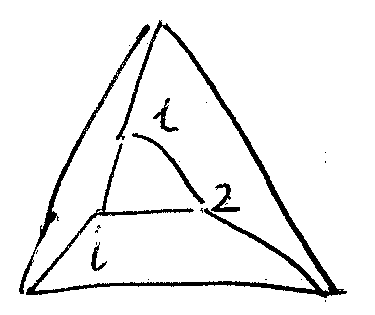
\includegraphics[width=\linewidth]{figures/gelfand-p001488-top-triangle-graph-original.png}
\par\smallskip{\footnotesize Оригинал рукописного рисунка: GELFAND-P001488\par}
\end{minipage}\hfill
\begin{minipage}[c]{0.48\linewidth}\centering
\resizebox{\linewidth}{!}{% Partial visible-stroke recreation. Endpoint hooks do not assert arrows; gaps remain open.
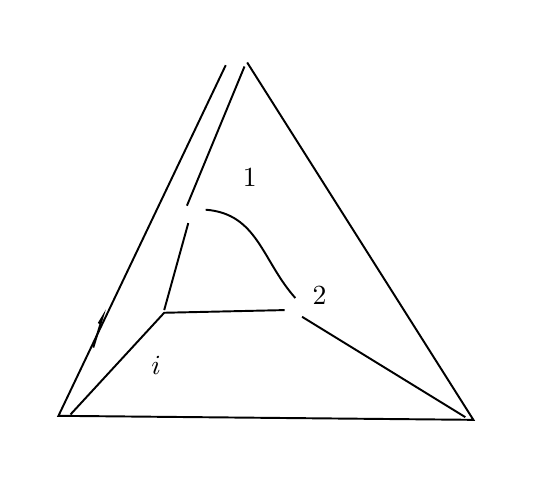
\begin{tikzpicture}[x=0.017cm,y=-0.017cm,line width=0.7pt]
\path[use as bounding box] (0,0) rectangle (375,315);
\draw (148,28)--(23,290)--(333,293)--(164,26);
\draw (162,29)--(119,133);\draw (120,146)--(102,211);
\draw (32,289)--(102,213)--(192,211);
\draw (133,136)..controls(172,139)and(175,174)..(200,202);
\draw (205,216)--(327,291);\draw (49,239)--(56,216)--(53,221);
\node at (166,112) {$1$};\node at (96,252) {$i$};\node at (218,200) {$2$};
\end{tikzpicture}
}
\par\smallskip{\footnotesize Частичное воссоздание; неясные направления и соединения остаются неустановленными.\par}
\end{minipage}\par\medskip


Рассмотрим
\begin{equation*}
Z_n=\sum_{\substack{\text{графы}\\ \text{с }n\\ \text{верш.}}}
\int\prod_{i=1}^{n}d\vec{x}_i\,
e^{-\sum_{\langle ij\rangle}(x_i^{\mu}-x_j^{\mu})^2}
\tag{9}
\end{equation*}

$\langle ij\rangle$ — ближайшие соседи в графе;

внутр. вершины

(10) Интеграл в (9) равен $\det^{-D/2}(3I-G)$.

[От $G$ проведён штрих к пояснению:]
Матр. [зачёркнуто:
\RussianUnclear{GELFAND-P001488}{middle-cancelled-incidence}{инцидентности?}]
смежности вершин

($G_{ij}=1\Longleftrightarrow i,j$ соед. ребром

$G_{ij}=0$
\RussianUnclear{GELFAND-P001488}{middle-overdrawn-equivalence}{густо обведённый / зачёркнутый знак $\Longleftrightarrow$}
в прот. случае).

[В первой строке знак $G$ переправлен:
\RussianUnclear{GELFAND-P001488}{middle-overdrawn-matrix-symbol}{прежний знак $E$ / $G$?}.]

\underline{\underline{Капранов Миша.}}

\underline{О раб. [зачёркнуто: Б.-Г.-Г.] о $\mathcal{D}$-модулях.}
[Под зачёркнутым сокращением вставлено: Берншт.-Гельф.-Гельф.]

$V$ — векторное [зачёркнуто:
\RussianUnclear{GELFAND-P001488}{lower-cancelled-space-token}{пр / неразборчивый короткий знак}]
пространство, $P(V)$ — его проективизация.

$O(-1)$ — рассл. на $P(V)$ (основное);
[над «рассл.» вставлено: тавтологическое]

[Справа:]
\begin{equation*}
O(-1)\subset P(V)\times V
\end{equation*}
[Под $O(-1)$:
\RussianUnclear{GELFAND-P001488}{lower-tautological-annotation}{два вертикальных дугообразных штриха: вертикальное равенство / двойная помета?},
справа от них $\{(\ell,x)\mid x\in\ell\}$.]

Точки $P(V)$ — это прямые $\ell$ в $V$, проход. через $0$;
она и явл. слоем над $\ell$.

$O(-k)=O(-1)^{\otimes k}$, $k>0$;

$O(+k)$ — двойств. расслоение к $O(-k)$.

\underline{Способ констр. новых расслоений:}

$\Lambda(V)$ — внешняя алгебра над $V$;

$\Lambda^k(V)$ — однородная степени $k$ часть $\Lambda(V)$.

Рассматриваются модули над $\Lambda(V)$ с градуировкой.
\begin{equation*}
\{\ldots\ M_{-1};\ M_0;\ M_1;\ \ldots\},
\qquad \Lambda^kM_i\subset M_{i+k}.
\end{equation*}

\underline{Упражнение к след. разу:} написать ответы для
[зачёркнуто:
\RussianUnclear{GELFAND-P001488}{bottom-cancelled-exercise-symbol}{$M$ / $V$?}]
$\dim V=1$ и $2$.


\RussianSourceFrame{GELFAND-P001489}{unlabelled}
$V\ni v$, $v^2=0$ в $\Lambda(V)$.

Рассм. умножение на $v$:
\begin{equation*}
(1)\qquad
\ldots\to M_{-1}\overset{v}{\longrightarrow}M_0
\overset{v}{\longrightarrow}M_1\overset{v}{\longrightarrow}M_2\to\ldots
\end{equation*}
$v^2=0\ \Rightarrow$ получ. комплекс.
\begin{equation*}
\operatorname{Ker}v\supset\operatorname{Im}v,
\end{equation*}
[Зачёркнуто справа от формулы:
\RussianIncomplete{GELFAND-P001489}{cancel-after-image}{Зачёркнутый фрагмент не удаётся прочесть.}]

Рассм. [Зачёркнуто:
\RussianIncomplete{GELFAND-P001489}{cancel-before-bundle}{Зачёркнутый фрагмент между «Рассм.» и «расслоение» не удаётся прочесть.}]
расслоение
\begin{equation*}
v\longmapsto
\frac{\operatorname{Ker}\{v:M_0\to M_1\}}
{\operatorname{Im}\{v:M_{-1}\to M_0\}},\qquad v\ne0.
\end{equation*}
Это «расслоение», а точнее, «пучок» над $\mathbb P(V)$.

\underline{Примеры.}\newline
\underline{модулей}

1). Сам $\Lambda(V)$
\begin{equation*}
\underset{0}{\mathbb C}\overset{v}{\longrightarrow}
\underset{1}{V}\overset{v}{\longrightarrow}
\underset{2}{\Lambda^2V}\overset{v}{\longrightarrow}
\ldots\overset{v}{\longrightarrow}\underset{N}{\Lambda^NV}
\end{equation*}
Ей соотв. нулевое расслоение; $\operatorname{Ker}v=\operatorname{Im}v$.

2) Обрезанная алгебра $\Lambda$, т.е. $\Lambda^{\ge k}(V)$

(оставл. только компоненты степеней $\ge k$).
\begin{equation*}
\{0;\ \Lambda^kV\overset{v}{\longrightarrow}\Lambda^{k+1}V;\ \ldots\}
\end{equation*}
[Под стрелкой зачёркнут знак:
\RussianUnclear{GELFAND-P001489}{truncated-arrow-cancel}{$v$ / $k$.}]

Расслоение:
\begin{equation*}
\operatorname{Ker}\{v:\Lambda^kV\to\Lambda^{k+1}V\}
=\Omega^{k-1}_{\mathbb P(V)}\otimes O(k)
\end{equation*}
[Под $\Omega^{k-1}_{\mathbb P(V)}$ проведена черта к подписи:
$(k-1)$-формы на $\mathbb P(V)$.]

3) Пусть $V$ — симплектич. пр-во, $[\ ,\ ]$ — $2$-форма;
[Над «$2$-форма» вписано и соединено фигурной скобкой:
\RussianUnclear{GELFAND-P001489}{symmetry-note}{симм.}]

рассм. модуль
\begin{equation*}
0\to\underset{-1}{\mathbb C}\overset{v}{\longrightarrow}
\underset{0}{V}\overset{v}{\longrightarrow}\underset{1}{\mathbb C}\to0
\end{equation*}
\begin{equation*}
v:w\longmapsto[v,w]
\end{equation*}
\begin{equation*}
v\longmapsto v^{\perp}/\mathbb Cv,
\qquad\perp\text{ — ортог. отн. }[\cdot,\cdot]
\end{equation*}

\underline{Теорема.} Всякое алгебраическое векторное расслоение
над $\mathbb P(V)$ происходит у некоторого $\Lambda(V)$-модуля
\begin{equation*}
E=\frac{\operatorname{Ker}\{v:M_0\to M_1\}}
{\operatorname{Im}\{v:M_{-1}\to M_0\}},
\quad\text{а другие факторы }=0.
\end{equation*}


\RussianSourceFrame{GELFAND-P001490}{92}
\underline{Док-во} см. в приложении С. Гельфанда
к книге \underline{Оконек} и др. «Расслоения над проект. пр-вом».

\underline{Формулир.}: заметка в ФА в 1978 году.

В док-ве использ. \underline{производные} категории. Можно ли этого
избежать? С. Гельфанд считает, что нельзя.

\underline{Рез. Капранова}: описание рассл. над квадрикой
в $\mathbb P(V)$.
\begin{equation*}
V,\quad\langle\ \rangle,\qquad
\mathbb P(V)\supset Q=\{v:\langle v,v\rangle=0\}
\end{equation*}
[Под $\langle\ \rangle$ проведена черта к подписи: симм. форма.]

Строим град. ал. Клиффорда [Над строкой вписано со скобкой: $A(V)$],
порожд. образующими
\begin{equation*}
v,\quad\operatorname{deg}v=1\text{ и }h,\quad\operatorname{deg}h=2
\end{equation*}
[Под $h$ проведена черта к подписи: фиксир.]
\begin{equation*}
vv'+v'v=\langle v,v'\rangle h
\end{equation*}
В \RussianUnclear{GELFAND-P001490}{basis-abbreviation}{ортон. / ортог.}
базисе $e_1,\ldots,e_r$
\RussianUnclear{GELFAND-P001490}{clifford-normalization}{$e_i^2=h,\qquad
e_ie_k=-e_ke_i,\quad i\ne k.$}
При $r=3$ это $\approx$ кватернионы.

\begin{equation*}
\langle v,v\rangle=0\ \Rightarrow\ v^2=0
\end{equation*}
и строим такое же расслоение.

Тогда верна такая же теорема.

